% !TEX root = ../../../main.tex
% 来源：中学数学实验教材·第三册（高中数学）
% 章节：二次函数 / 多项式函数的增减性
% 原始文件：5.tex，行 2573-2604
% 类型：tikz
% ---
    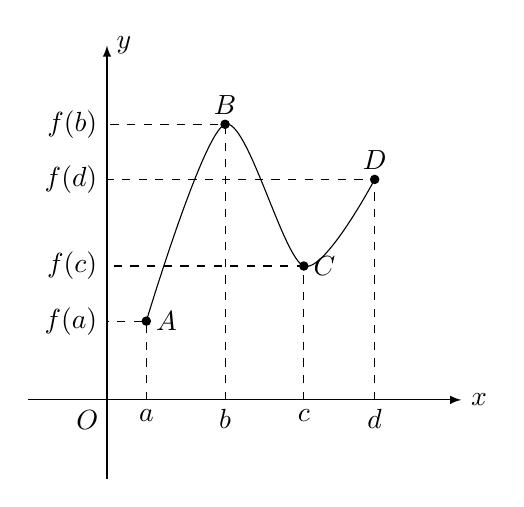
\begin{tikzpicture}[>=latex, scale=1]
        \draw[->] (-1,0)--(4.5,0)node[right]{$x$};
        \draw[->] (0,-1)--(0,4.5)node[right]{$y$}  ;
        \node at (-.25,-.25){$O$};
\foreach \x/\y in {.5/1,1.5/3.5,2.5/1.7,3.4/2.8}
{
    \draw[dashed] (\x,0)--(\x,\y)--(0,\y);
    \draw (\x,\y)[fill=black] circle(1.5pt);
}

\draw plot[smooth, very thick] coordinates{(.5,1) (1.5,3.5) (2.5,1.7) (3.4,2.8)};

\foreach \x\xtext in {.5/a,1.5/b,2.5/c,3.4/d}
{
    \node at (\x, 0) [below]{$\xtext$};
}

\foreach \ytext\y in {f(a)/1,f(b)/3.5,f(c)/1.7,f(d)/2.8}
{
    \node at (0,\y) [left]{$\ytext$};
}

\foreach \x/\xtext in {{1.5,3.5}/B, {3.4,2.8}/D}
{
    \node at (\x) [above]{$\xtext$};
}
\foreach \x/\xtext in {{.5,1}/A, {2.5,1.7}/C}
{
    \node at (\x) [right]{$\xtext$};
}

    \end{tikzpicture}
